%Параметры страницы для большей схожести с веб-версией
\documentclass[12pt]{article}
\usepackage[total={170mm,230mm}]{geometry}

\usepackage{cmap}
%\usepackage{hyperref}
\usepackage[utf8]{inputenc}
\usepackage[T2A]{fontenc}
\usepackage[russian]{babel}

\usepackage{graphicx}
\usepackage{xcolor}
\usepackage{amssymb}
\usepackage{amsfonts}
\usepackage{amsmath}
\usepackage{amsthm}
\usepackage{physics}
\usepackage{wrapfig}
\usepackage{cancel}
\usepackage{pdfpages}
\usepackage{hyperref}
\newtheorem{definition}{Опредление}[section]
\newtheorem{theorem}{Теорема}[section]
\newtheorem{axiom}{Аксиома}[section]
\newtheorem{hypothesis}{Гипотеза}[section]

\usepackage{pgfplots}
\pgfplotsset{width=7cm,compat=newest}

\usepackage{amsmath}
\DeclareMathOperator\arctanh{arctanh}

\usepackage{amsmath}
\DeclareMathOperator\arccosh{arccosh}

\usepackage{amsmath}
\DeclareMathOperator\const{const}

\title{Последовательности и их пределы}
\author{Алексей Савватеев \and Александр Тонис}

\begin{document}
\maketitle
\begin{abstract}
В настоящей лекции рассмотрены понятия последовательности и её предела. Приведён пример вычисления предела последовательности. Исследован бином Ньютона и выведена формула для биномиальных коэффициентов. Кроме того, затронуты рекуррентные последовательности и продемонстрирован пример хаотического поведения последовательности. 
\par
Конспектировал Александр Козлов. 
\end{abstract}
\newpage
\tableofcontents
\newpage
\section{Последовательность}
\subsection{Определение}
Рассмотрим такой объект, как последовательность. Дадим формальное определение.
\begin{definition}
Последовательностью действительных чисел называют отображение множетсва всех натуральных числе во множество действительных чисел:
\begin{equation}
    \mathbb{N}\longrightarrow\mathbb{R}.
\end{equation}
\end{definition}
Данное определение имеет обобщение. Так, например, последовательностью элементов множества $X$ называют отображение натуральных чисел во множество $X$:
\begin{equation}
    \mathbb{N}\longrightarrow X.
\end{equation}
То есть последовательность -- это просто пронумерованный натуральными индексами набор элементов множества $X$. Обозначают последовательность элементов множества $X$ следующим образом:
\begin{equation}
    \qty{a_n}_{n=0}^\infty = a_0, a_1, a_2, \ldots \in X.
\end{equation}
\subsection{Качественное представление о сходимости и расходимости}
По аналогии с рядами с неотрицательными членами для последовательностей можно ввести понятия сходимости и расходимости. Рассмотрим геометрические иллюстрации к последовательностям точек плоскости\footnote{Плоскость является декартовым произведенением множеств действительных чисел $\mathbb{R}\cross \mathbb{R}$, что значит, что каждая точка плоскости отвечает паре действительных чисел.}.
\par
Сперва обратимся к сходимости (см. рис. \ref{fig:1}). Видно, что с ростом номера элементы последовательности начинают располагаться всё в более и более малых кругах. Наблюдается сгущение элементов последовательности. 
\begin{figure}[ht]
    \centering
    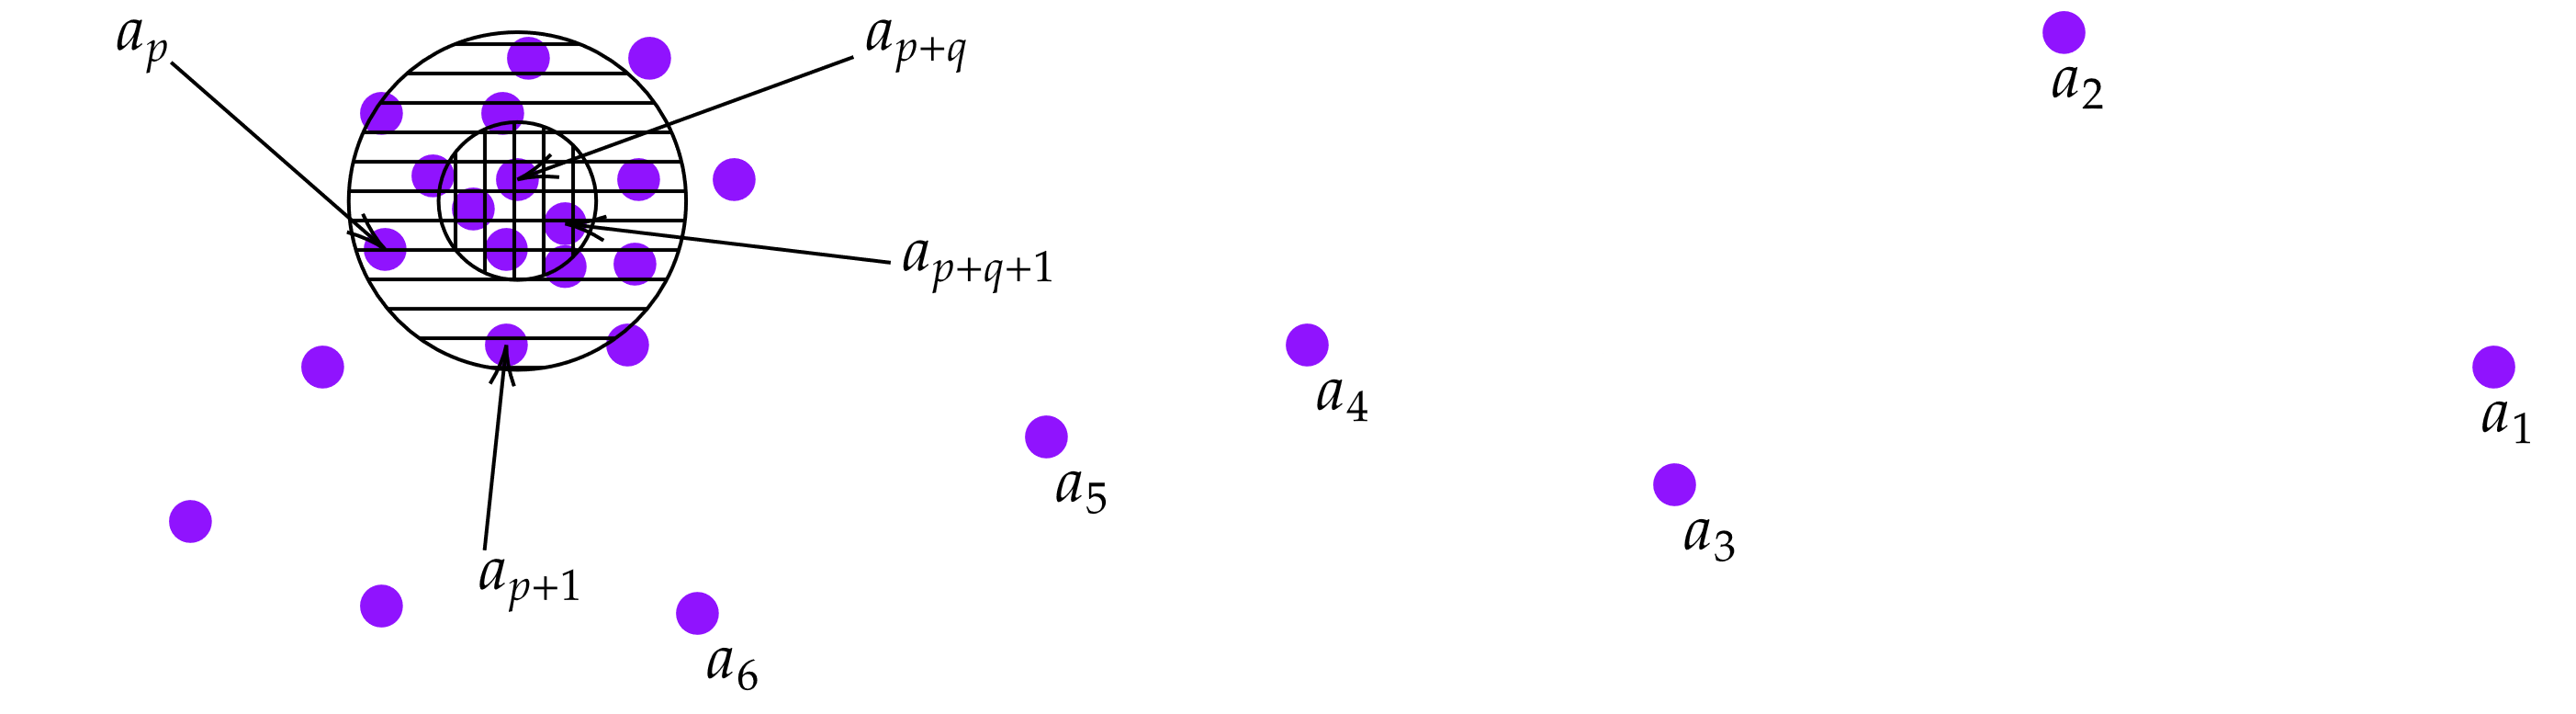
\includegraphics[width = 1\textwidth]{fig1.png}
    \caption{Геометрическая иллюстрации сходящейся последовательности точек плоскости. Начиная с номера $p$ элементы последовательности лежат в круге, закрашенном горизонтальной штриховкой. Начиная с номера $p+q$ элементы последовательности начинают лежать в меньшем круге, закрашенном вертикальной штриховкой.}
    \label{fig:1}
\end{figure}
То есть то, что последовательность сходится, означает, что флуктуации точек последовательности должны затухать, хотя бы с какого\--то элемента. Это как раз и означает, что можно найти настолько большой номер элемента последовательности, что каждый последующий элемент не покинет данного сколь угодно малого круга с центром в точке, к которой последовательность сходится.
\par
Теперь рассмотрим расходимость. Существуют различные проявления расходимости. Самый простой из них~\----~элементы последовательности, начиная с какого\--то номера, начинают уходить на бесконечность (см. рис. \ref{fig:2}). Элементы не накапливаются безгранично ни в одном круге конечного радиуса.
\begin{figure}[ht]
    \centering
    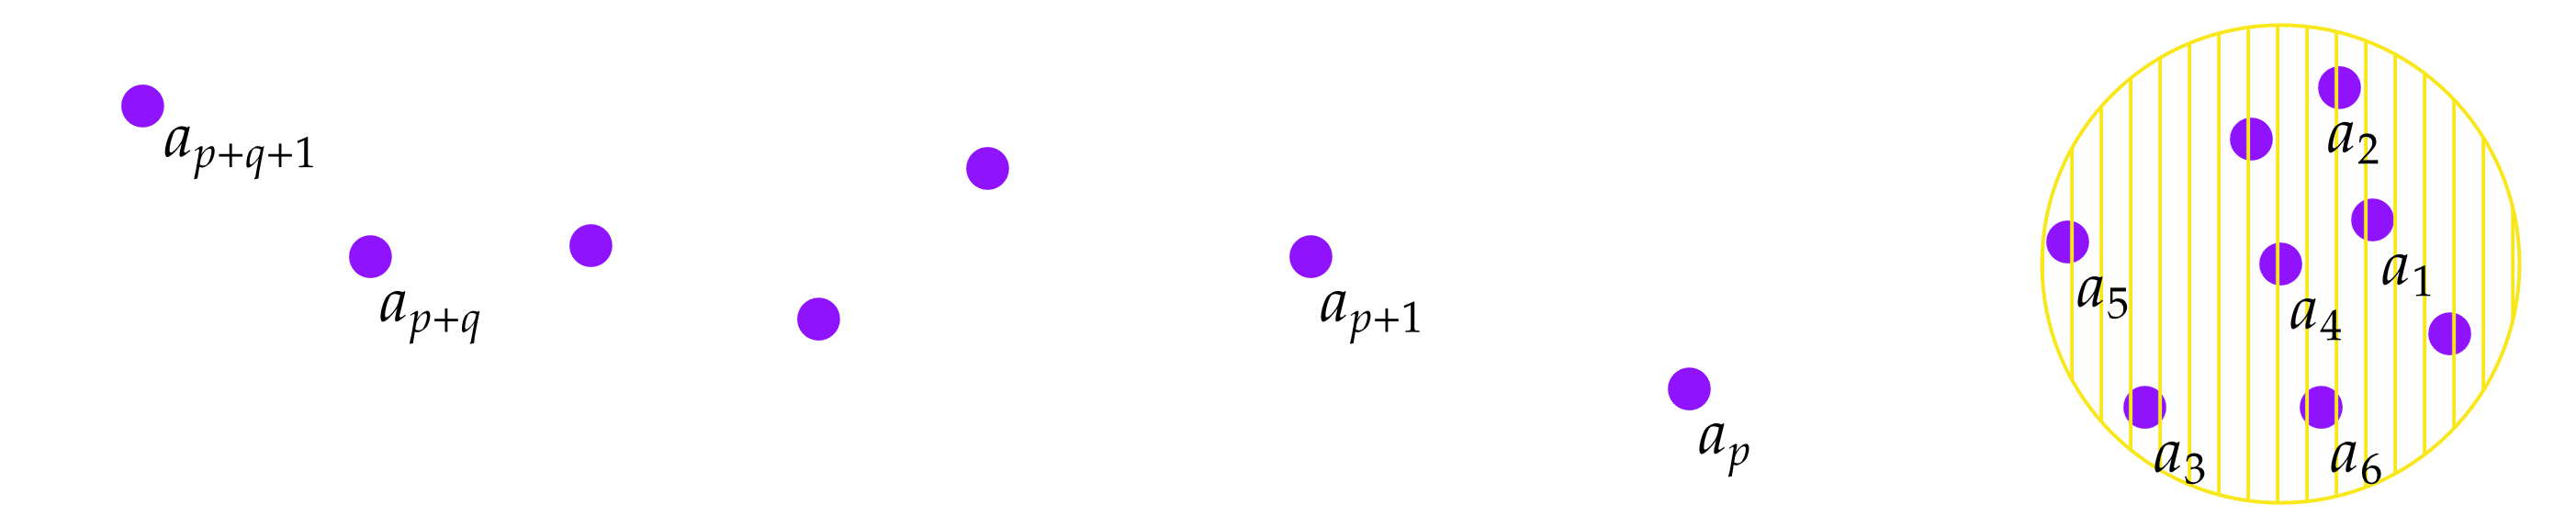
\includegraphics[width = 1\textwidth]{fig2.png}
    \caption{Геометрическая иллюстрации расходящейся последовательности точек плоскости. Начиная с номера $p$ элементы последовательности покидают круг, закрашенный жёлтой штриховкой, и начинают удаляться от прочих элементов на бесконечность.}
    \label{fig:2}
\end{figure}
\par
Примером расходящейся последовательности действительных чисел может служить следущая последовательность:
\begin{equation}
    0,1,2,3,4,\ldots
\end{equation}
Рассматриваемый пример является результатом отображения множества натуральных чисел в себя же. Такая последовательность безгранично растёт и поэтому расходится.
\par
Кроме данного типа расходимости можно выделить и другой~\----~расходимость в конечном пространстве (см. рис. \ref{fig:3}). Она отлична от прошлого типа тем, что последовательность локализована и не выходит за пределы некоторой территории. Причина данной расходимости, как и в прошлый раз, кроется в том, что флуктуации элементов последовательности не заухают. То есть нельзя найти такой номер элемента последовательности, начиная с которого элементы будут накапливаться в сколь угодно малый круг.
\begin{figure}[ht]
    \centering
    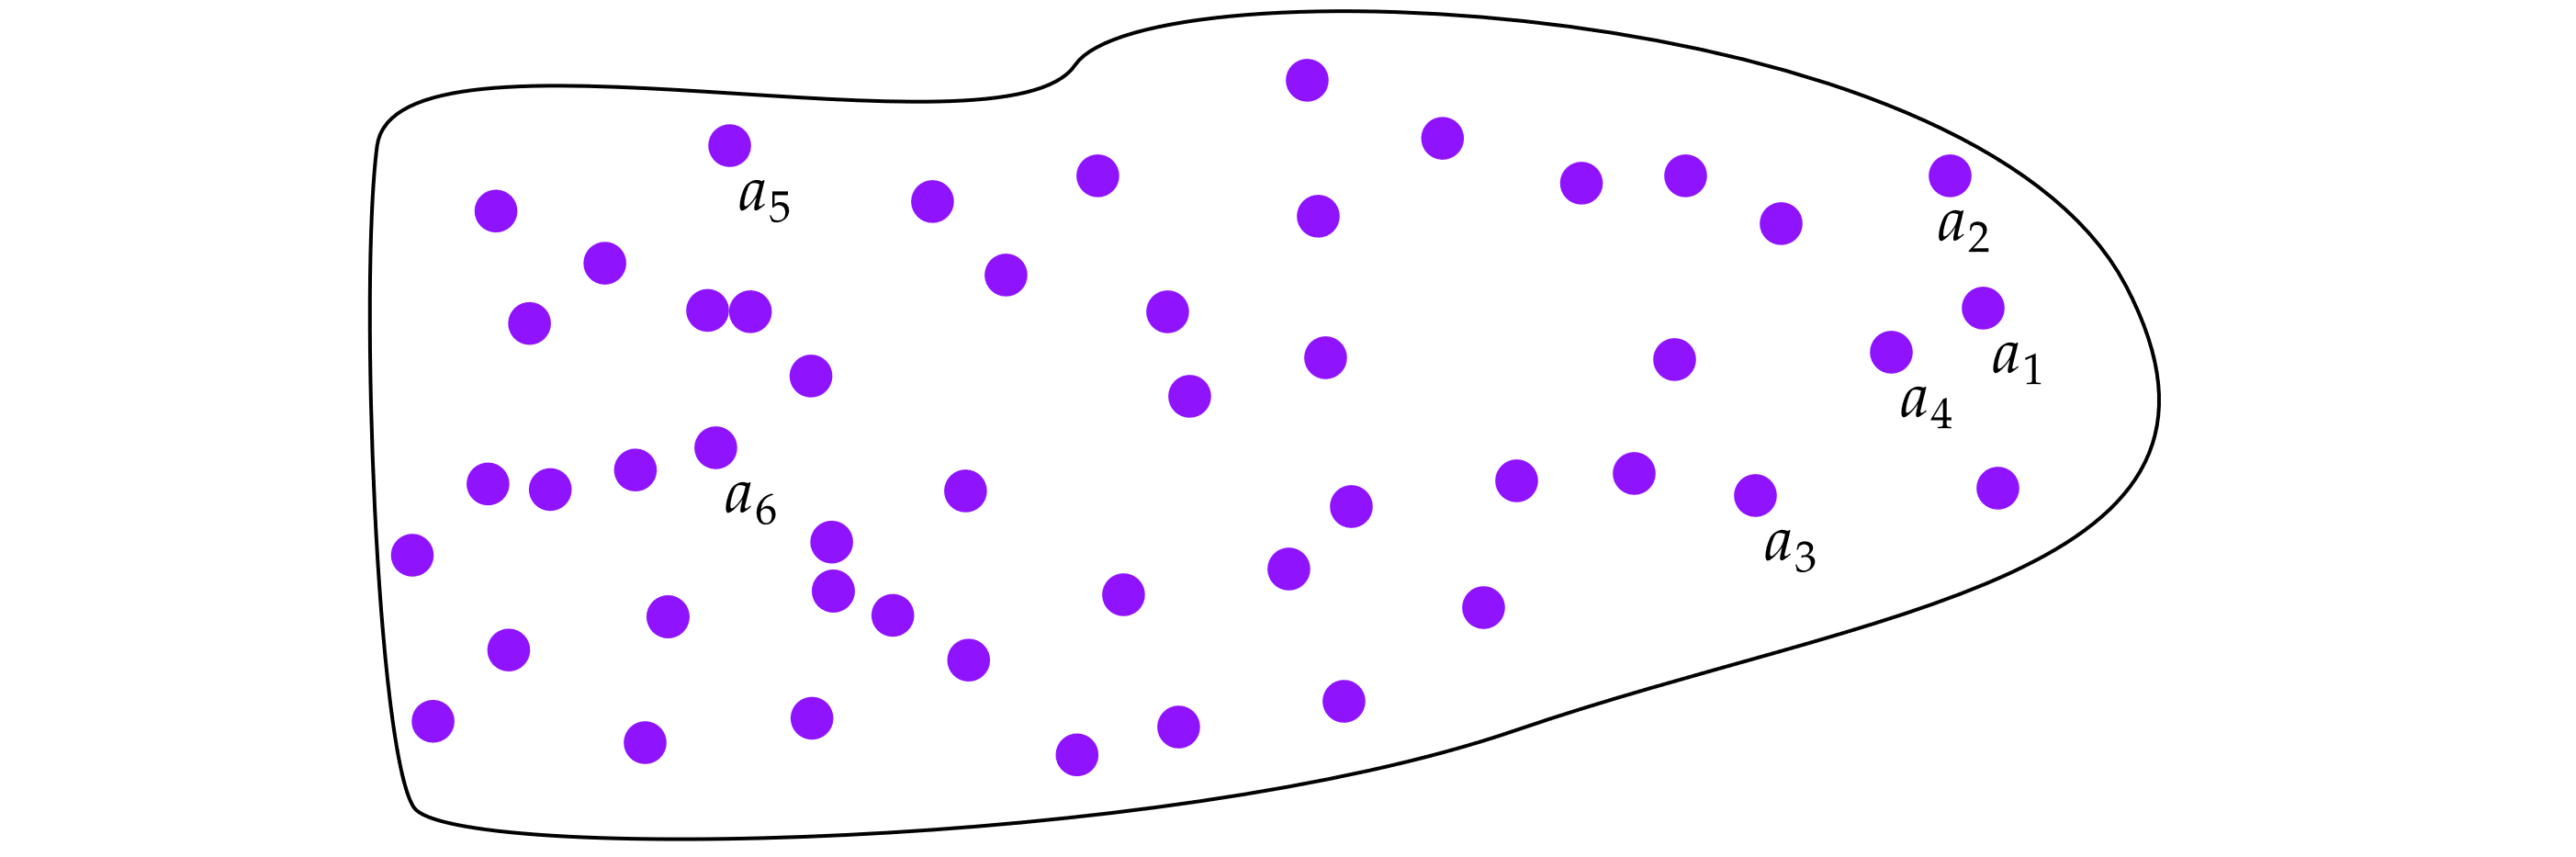
\includegraphics[width = 1\textwidth]{fig3.png}
    \caption{Геометрическая иллюстрации расходящейся последовательности точек плоскости в ограниченном пространстве.}
    \label{fig:3}
\end{figure}
\section{Сходимость последовательности}
Снова рассмотрим сходящуюся последовательность точек плоскости. Напомним, что сходимость означает, что флуктуации элементов последовательности затухают. Чтобы можно было говорить о величине данных флуктуаций, введём понятие расстояния между точками на плоскости. Расстояние между точками $x$ и $y$ будет вычисляться следующим образом:
\begin{equation}
    \rho\qty(x,y)=\norm{x-y} = \sqrt{\qty(x_1 - y_1)^2 + \qty(x_2 - y_2)^2}.
\end{equation}
Это не что иное, как длина вектора $x-y$, где $x$ и $y$~\----~радиус\--вектора. Здесь использована теорема Пифагора, доказательство которой было дано ранее \cite{pif}.
\par
Кроме того, для дальнейших рассуждений нужно ввести понятие диаметра множества. Но перед тем, как дать строгое определение, рассмотрим некоторые примеры. Во\--первых, рассмотрим множество точек плоскости, оганиченных ромбом (см. рис. \ref{fig:5}). Диаметром данного множества будет длина наибольшей диагонали ромба. То есть диаметром является наибольшее расстояние между двумя элементами множества.
\begin{figure}[ht]
    \centering
    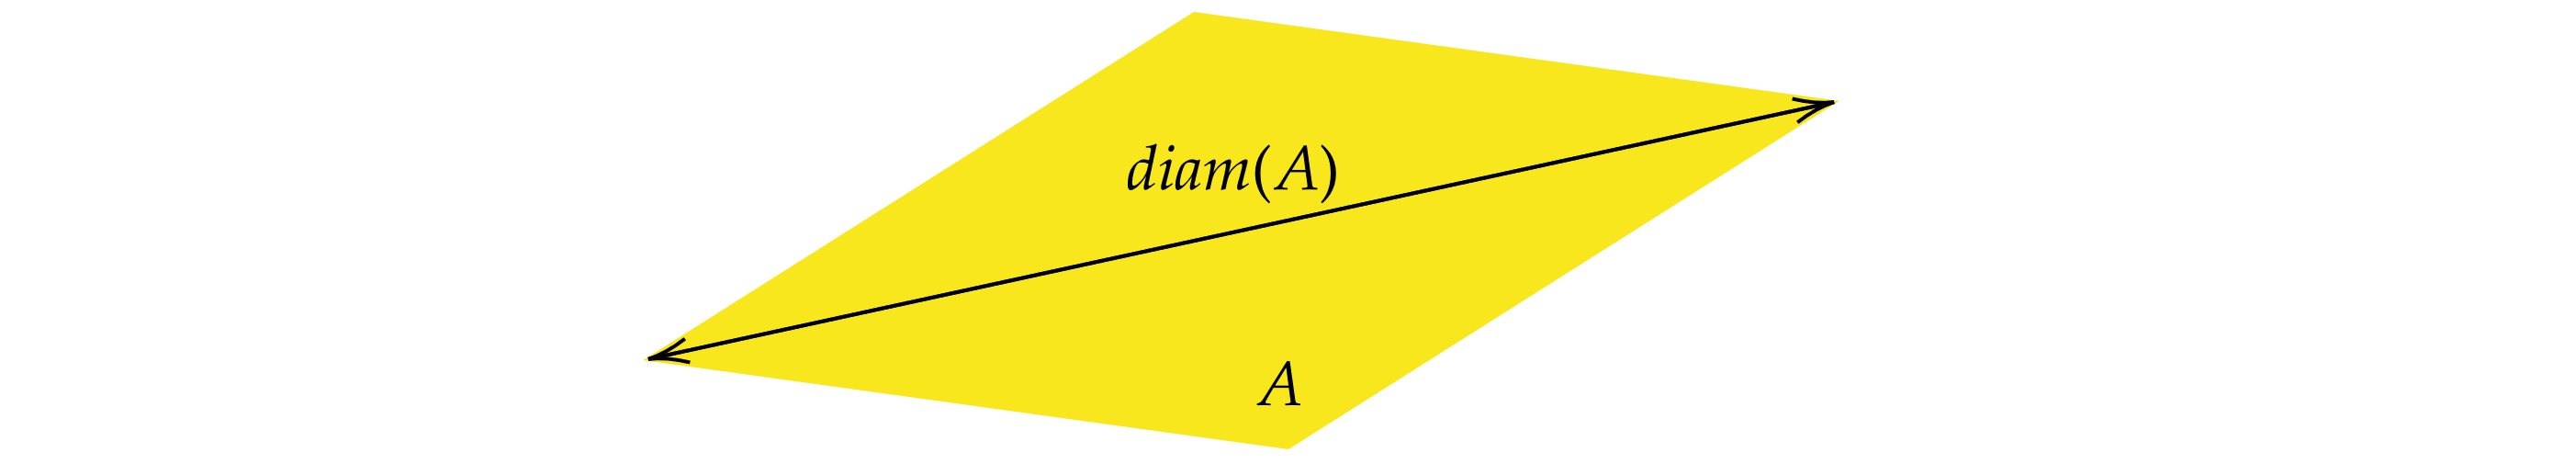
\includegraphics[width = 1\textwidth]{fig5.png}
    \caption{Множество точек плоскости, оганиченных ромбом. Множество именуется $A$. Диаметром его является длина наибольшей диагонали ромба.}
    \label{fig:5}
\end{figure}
\par
Но такое понимание диаметра множества не совсем верно, продемонстрируем это на втором примере. Рассмотрим открытый круг $K$ (круг с изъятой границей~\----~окружностью). Для множества $K$ не удаётся найти максимального расстояния между двумя любыми элементами множества. Причина этого кроется в открытости множества. То есть нет никакой границы, принадлежащей множеству $K$, перейдя которую мы окажемся за пределом $K$. Поэтому для любой пары точек из $K$ найдётся другая пара точек из $K$, расстояние между которыми больше расстояния между точками первой пары (см. рис. \ref{fig:6}.a). То есть во множестве $K$ можно организовать последовательность точек, которые безгранично приближаются к окружности, ограничивающей множество $K$, но которые никогда не покинут множество $K$ (см. рис. \ref{fig:6}.b).
\begin{figure}[ht]
    \centering
    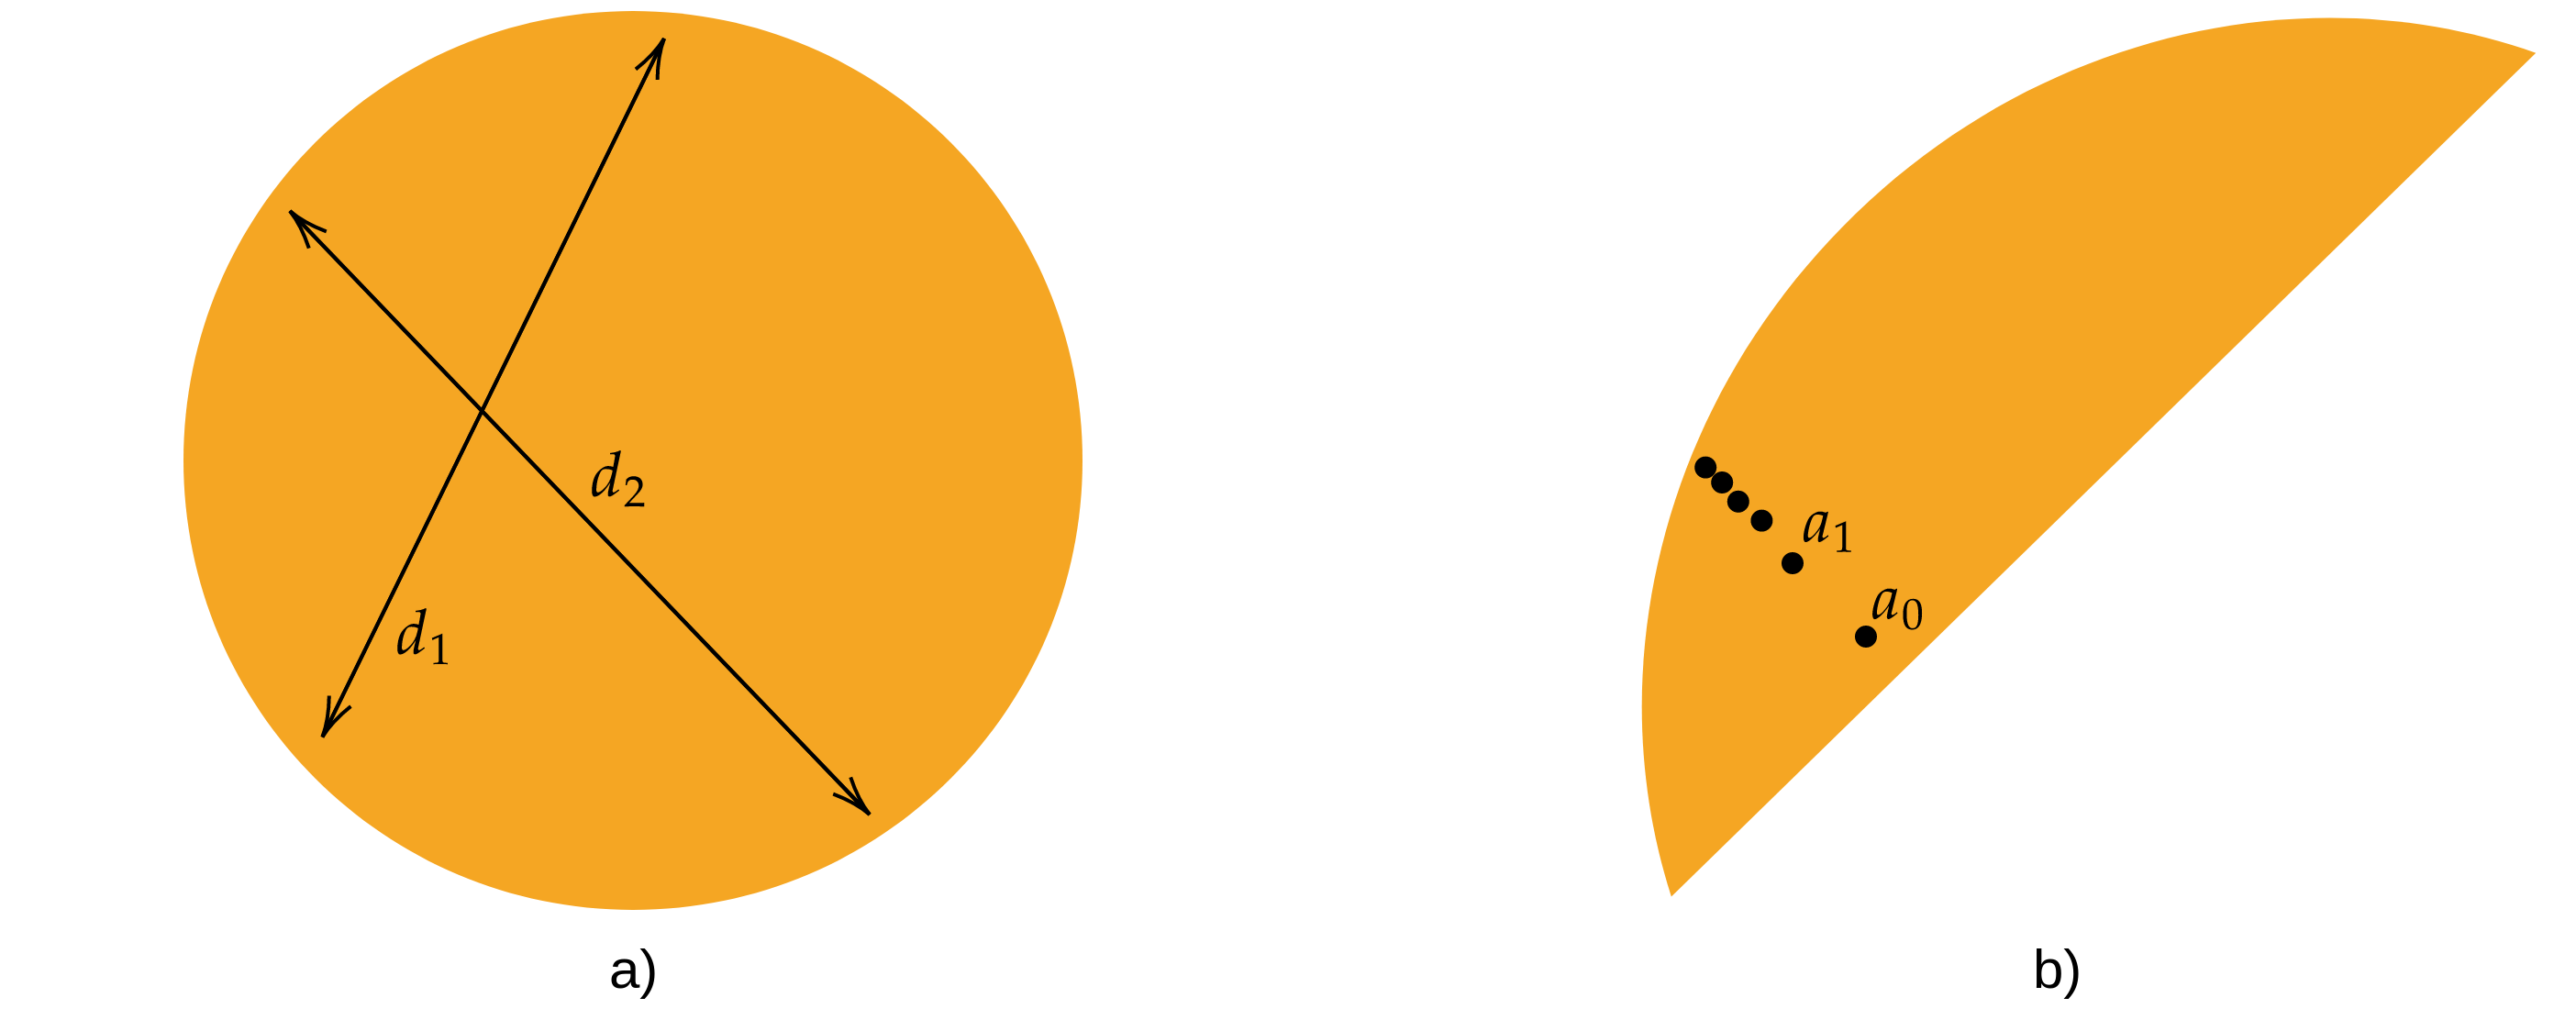
\includegraphics[width = 1\textwidth]{fig6.png}
    \caption{Иллюстрация открытого круга, сам круг обозначен оранжевым.\\ a) Для двух точек, между которыми расстояние $d_1$ нашлась другая пара точек, расстояние между которыми $d_2 > d_1$.\\ b) Показана последовательность точек $\qty{a_k}_{k=0}^{\infty} \in K$, безгранично приближающихся к окружности, ограничевающей открытый круг.}
    \label{fig:6}
\end{figure}
\par
Данное обстоятельство наводит на мысль, что нужно использовать некоторое обобщение понятия максимума. Таким понятием является супремум. Действительно, наиболее ясным ответом на вопрос о диаметре открытого круга является диаметр окружности, ограничевающей круг, кроме того, такой же ответ даёт поиск супремума расстояний между парой точек открытого круга.
\par
Данные соображения навели нас на определения диаметра множества, которое сформулируем следующим образом.
\begin{definition}
Диаметром множества $A$ называется супремум расстояний между двумя элементами множества $A$:
\begin{equation}
    diam\qty(A) = \sup\qty{\norm{x-y}\eval x,y\in A}.
\end{equation}
\end{definition}
Так, например, для неограниченных множеств диаметр будет равен бесконечности. Кроме того, в дальнейших рассуждениях пригодится очевидный факт. Если имеется два множества $A$ и $B$ таких, что $B \subset A$, то $diam\qty(B) \le diam\qty(A)$.
\par
Попробуем сформулировать в терминах диаметра понятие сходимости последовательности. Будем использовать тот факт, что в сходящихся последовательностях с увеличением индекса амплитуда флуктуаций элементов последовательности затухает. Тогда выходит, что, вроде бы, должна быть справедлива следующая гипотеза.
\begin{hypothesis}
Последовательность сходится, если диаметр остаточной последовательности (то есть последовательности без первых $n$ членов)
\begin{equation}
    diam\qty{a_n, a_{n-1}, \ldots}
\end{equation}
неограниченно приближается к $0$.
\end{hypothesis}
То есть мерой флуктуаций элементов последовательности становится диаметр остаточной последовательности, и если он неограниченно приближается к нулю (то есть флуктуации затухают), то последовательность сходится. Вроде бы всё понятно. Но остаётся два подводных камня.
\par
У нас ещё нет строгого определения того, что значит, что последовательность действительных чисел неограниченно приближается к $0$. На прошлой лекции было дано понятие неограниченного приближение частичных сумм ряда к сумме ряда, неограниченное стремление к $0$ является очень близким понятием. Строгое математическое определение будет дано ниже.
\par
Вторая проблема заключается в полноте множества, последовательность элементов которого мы рассматриваем. Если, например, множество точек плоскости не полно, то нельзя гарантировать, что существует точка, к которой стягивается множество остаточной последовательности. То есть может случиться такая ситуация, что диаметр множества остаточной последовательности стремится к нулю, но нет точки, к которой множество остаточной последовательности стягивается, поэтому говорить о сходимости в таком случае не приходится, ибо это лишено смысла. Чтобы гарантировать наличие такой точки для последовательностей на плоскости $\mathbb{R}\cross \mathbb{R}$, надо опять же использовать аксимому полноты вещественных чисел\footnote{Напомним, что каждая точка на плоскости есть не что иное, как пара действительных чисел, поэтому полнота действительных чисел обеспечит и полноту множества $\mathbb{R}\cross \mathbb{R}$.}.
\par
В данном месте важно отметить, что такая последовательность, что диаметр множества её остаточных элементов неограниченно приближается к нулю, называется \emph{фундаментальной}.

\section{Предел последовательности}
\subsection{Определение сходящейся последовательности}
Дадим строгое математическое определение последовательности на плоскости, сходящейся к точке $\overline{x}$. Для этого предварительно введём обозначения для круга с центром в точке $M$ и радиусом $R$:
\begin{equation}
    D_M^R.
\end{equation}
\begin{definition}\label{def:31}
Последовательность точек плоскости $\qty{a_n}_{n=0}^\infty \in \mathbb{R} \cross \mathbb{R}$ называют сходящейся к точке $\overline{x} \in \mathbb{R} \cross \mathbb{R}$, что обозначают следующим образом:
\begin{equation}
   {a_n} \overset{}{\underset{n \rightarrow \infty}{\longrightarrow}} \overline{x},
\end{equation}
если 
\begin{equation}
    \forall \varepsilon > 0\ \exists N \in \mathbb{N} \eval \forall n \ge N \Longrightarrow a_n \in D_{\overline{x}}^{\varepsilon}.
\end{equation}
\end{definition}
То есть последовательность называется сходящейся к точке $\overline{x}$, если для сколь угодно малого круга с центром в точке $\overline{x}$ можно указать номер члена последовательности, начиная с которого все элементы последовательности лежат в этом малом круге. Это как раз и означает, что диаметры остаточных последовательностей неограниченно убывают к нулю.
\par
Стоит заметить, что определение сходящейся последовательности действительных чисел даются аналогичным образом~\----~в определении \ref{def:31} нужно лишь заменить круг $D_{\overline{x}}^{\varepsilon}$ на интервал ($\overline{x}-\varepsilon,\overline{x}+\varepsilon$).
\subsection{Ряды и последовательности}
Сравним определение суммы ряда \cite{sum}, когда ряд сходится, с определением сходящейся последовательности. Рассмотрим сначала сходящейся ряд с неотрицательными членами (см. рис. \ref{fig:7}). Пускай сумма ряда равна $A$:
\begin{equation}
    \sum_{n=0}^\infty a_n = A.
\end{equation}
Напомним, что это значит, что число $A$ является наименьшим из всех чисел, которые больше любой из частичных сумм ряда, то есть $A$ является супремумом частичных сумм ряда.
\begin{figure}[ht]
    \centering
    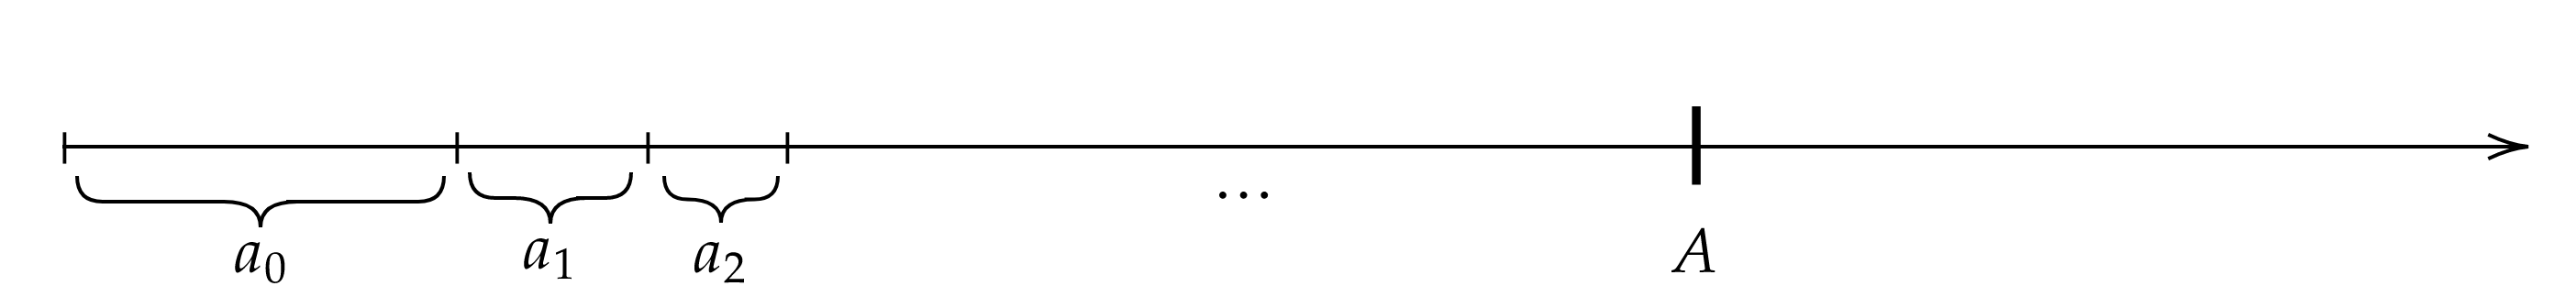
\includegraphics[width = 1\textwidth]{fig7.png}
    \caption{Иллюстрация к суммированию ряда с неотрицательными слагаемыми $\sum a_n$. За $A$ обозначена сумма ряда.}
    \label{fig:7}
\end{figure}
\par
То есть данные свойства числа $A$ можно записать следующим образом:
\begin{equation}\label{eq:10}
\forall n \Longrightarrow \sum_{k=0}^n a_k < A;
\end{equation}
\begin{equation}
\forall \varepsilon > 0\ \exists n \eval \sum_{k=0}^n a_k> A - \varepsilon.
\end{equation}
Фактически здесь написанно, что $A$ является пределом последовательности частичных сумм. Сравним это с тем, что мы требуем от сходящихся последовательностей.
\begin{figure}[ht]
    \centering
    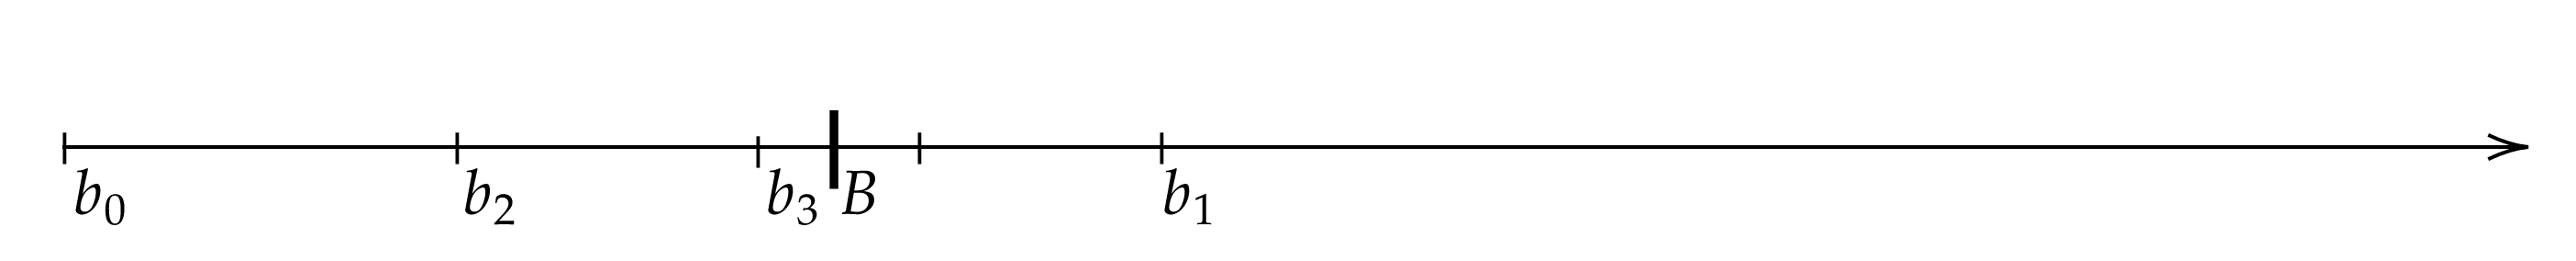
\includegraphics[width = 1\textwidth]{fig8.png}
    \caption{Иллюстрация к сходящейся последовательности $\qty{b_k}_{k=0}^\infty$. За $B$ обозначен предел последовательности.}
    \label{fig:8}
\end{figure}
\par
Рассмотрим предел последовательности $\qty{b_k}_{k=0}^\infty$, которая сходится к числу $B$ (см. рис. \ref{fig:8}).
Вспомним, что это означает. Для удобства обозначения предела последовательности вводят такое обозначение:
\begin{equation}\label{eq:12}
    \lim_{k\rightarrow\infty}{b_k}.
\end{equation}
Итак, напоминаем определение. Последовательность действительных чисел $\qty{b_k}_{k=0}^\infty$ сходится к числу $B$ (что записывается, как (\ref{eq:12})), если
\begin{equation}
\forall \varepsilon > 0\ \exists N \in \mathbb{N} \eval \forall n \ge N \Longrightarrow b_n \in \qty(B - \varepsilon, B + \varepsilon).
\end{equation}
Если за $b_n$ обозначить частичные суммы ряда с неотричательными членами
\begin{equation}
    b_n = \sum_{k=0}^n a_k,
\end{equation}
то для сходимости данного ряда нужно требовать меньше, чем для сходимости последовательности $b_n$. Нужно лишь потребовать (при выполнении (\ref{eq:10})), что \emph{одна} частичная сумма больше $A-\varepsilon$, в то время как для сходимости последовательности нужно требовать, чтобы \emph{все} $b_n$, начиная с какого\--то, лежали в $\varepsilon$\--окрестности предела. Но для ряда с неотрицательными слагаемыми это равноценные вещи, ибо если частичная сумма $n$ членов ряда больше какого\--то числа, то и следующие частичные суммы будут точно не меньше данного числа из\--за неотрицательности слагаемых.
\par
Последовательности, подобные последовательности частичных сумм, выделяются в отдельный класс последовательностей. Дадим их строгое определение.
\begin{definition}
Последовательность действительных чисел $\qty{b_k}_{k=0}^\infty$ называется монотонно неубывающей, если справедливо:
\begin{equation}
    b_m \le b_{m+1},
\end{equation}
где $m \in \mathbb{N}$.
\end{definition}
\begin{definition}
Последовательность действительных чисел $\qty{b_k}_{k=0}^\infty$ называется монотонно невозрастающей, если справедливо:
\begin{equation}
    b_m \ge b_{m+1},
\end{equation}
где $m \in \mathbb{N}$.
\end{definition}
Для монотонных последовательностей можно упростить определение предела. Так, например, для монотонно неубывающих последовательностей вводят следующее определение.
\begin{definition}
Монотонно неубывающая последовательность действительных чисел $\qty{b_k}_{k=0}^\infty$ называется сходящейся к числу $B$, если, во\--первых, выполняется требование:
\begin{equation}
    \forall k \Longrightarrow b_k < B.
\end{equation}
И, во\--вторых, верно:
\begin{equation}
    \forall \varepsilon > 0\ \exists N \in \mathbb{N}\eval b_N > B-\varepsilon.
\end{equation}
\end{definition}
Очевидно, что последовательность частичных сумм ряда с неотрицательными слагаемыми является монотонно неубывающей последовательностью. Поэтому и достаточно, чтобы лишь одна частичная сумма попала в $\varepsilon$\--окрестность суммы ряда при условии, что все частичные суммы ряда меньше суммы ряда.

\section{Классические пределы}
Существует сколько так называемых \emph{классических} пределов, знание которых значительно облегчает изучение математического анализа. Первым классическим пределом будем называть
\begin{equation}
    \lim_{n\rightarrow\infty}{\sqrt[n]{n}}=1.
\end{equation}
Вторым классическим пределом обозначим
\begin{equation}
    \lim_{n\rightarrow\infty} {\dfrac{x^n}{n!}} = 0,
\end{equation}
где на место $x$ можно поставить любое действительное число. 
\par
Чтобы взять данные пределы, нам нужно вспомнить комбинаторику. Величина $n!$ в комбинаторных терминах~\----~это количество способов, которыми можно перенумеровать $n$ предметов (либо же это количество возможных перестановок этих предметов, что то же самое). Кроме того, потребуется знание биномиальных коэффициентов, чему посвящён следующий раздел.

\section{Бином Ньютона}
Рассмотрим бином Ньютона, то есть зададимся вопросом о том, как произвести раскрытие скобок выражения
\begin{equation}\label{eq:23}
    \qty(a+b)^n.
\end{equation}
Обратимся сперва к простейщему примеру. Пускай $n=2$, тогда по формулам сокращённого умножения должно быть известно:
\begin{equation}
    \qty(a+b)^2 = a^2 + 2ab + b^2.
\end{equation}
Видно, что образовалось три типа слагаемых: произведение двух $a$, произведение двух $b$ и произведение $a$ и $b$. Последний тип слагаемых в сумме встречается два раза, поэтому он записан с фактором $2$.
\par
Идём дальше и рассматриваем $n=3$:
\begin{equation}
    \qty(a+b)^3 = a^3 + 3a^2b+3ab^2+b^3.
\end{equation}
В этот раз у нас образовалось четыре типа слагаемых. Угадывается закономерность~\----~количество типов слагаемых равно $n+1$.
\par
Вернёмся к общему случаю. При раскрытии скобок каждое слагаемое результурующей суммы будет иметь вид $a^{n-k}b^k$ с некоторым коэффициентом. Типов слагаемых опять будет $n+1$, потому что каждому типу слагаемых отвечает выражение $a^{n-k}b^k$, $k$ изменятеся от $0$ до $n$, то есть всего возможных значений $k$ будет $n+1$.
\par
Остался нерешённым вопрос о том, как определять коэффициенты перед $a^{n-k}b^k$. Для ответа на данный вопрос запишем выражение (\ref{eq:23}) в следующем виде:
\begin{equation}
    \qty(a+b)^n = \qty(a+b) \vdot  \qty(a+b) \vdot  \qty(a+b) \vdot \ldots \vdot  \qty(a+b),
\end{equation}
то есть в виде произведения $n$ скобок $\qty(a+b)$. При раскрытии скобок получим $2^n$ выражений, нам хочется узнать какую часть этих выражений будут составлять выражения $a^{n-k}b^k$ при заданном $k$. Такое слагаемое может быть сформировано, если из  всех $n$ скобок $k$ скобок отдаст $b$ на формирование рассматриваемого члена, а остальные отдадут $a$. \par
То есть нам нужно выделить из $n$ скобок $k$ скобок, откуда будет взято $b$. Сколько вариантов выбора первой из этих $k$ скобок существует? Очевидно, что $n$. Сколько вариантов выбора второй из этих $k$ скобок существует? Одна скобка из всех $n$ скобок уже нами занята, поэтому вариантов такого выбора остаётся лишь $n-1$. Продолжая такие рассуждения, приходим к выводу, что вариантов выбора $k$ скобок из $n$ скобок существует
\begin{equation}\label{eq:27}
    n \vdot \qty(n-1) \vdot \ldots \vdot \qty(n-k+1).
\end{equation}
Но данные рассуждения не учитывают того факта, что скобки для нас не различимы. То есть набор "первая скобка, вторая скобка, третья скобка, \ldots , последняя скобка"{} не отличим для нас от набора "вторая скобка, первая скобка, третья скобка, \ldots , последняя скобка"{}. Чтобы учесть идентичность скобок, нужно поделить выражение (\ref{eq:27}) на количество перестановок $k$ скобок, то есть на $k!$. Тогда получаем выражение, которое можно записать в более привычной форме:
\begin{equation}
\begin{split}
    &\dfrac{n \vdot \qty(n-1) \vdot \ldots \vdot \qty(n-k+1)}{k!}\\
    &= \dfrac{n \vdot \qty(n-1) \vdot \ldots \vdot \qty(n-k+1) \vdot \qty(n-k)!}{k! \vdot \qty(n-k)!}\\
    &=\dfrac{n!}{k! \vdot \qty(n-k)!}.
\end{split}
\end{equation}
Данное выражение именуют \emph{числом сочетаний из $n$ по $k$} и обозначают так:
\begin{equation}
    C_{n}^{k} = \dfrac{n!}{k! \vdot \qty(n-k)!}.
\end{equation}
Оно обозначает число способов выбора $k$ элементов из совокупности таких же $n$ элементов.
\par
Возвращаемся к биному Ньютона (\ref{eq:23}):
\begin{equation}
    \qty(a+b)^n = C_{n}^0 a^n + C_{n}^1 a^{n-1}b + \ldots + C_{n}^{n-1} a b^{n-1} + C_{n}^{n} b^n.
\end{equation}
Перед $a^n$ мы написали число сочетаний из $n$ по $0$, ибо оно равно числу способов, которыми можно выбрать $0$ скобок для $b$ и $n$ скобок для $a$. Перед $a^{n-1}b$ мы написали число сочетаний из $n$ по $1$, потому что именно столькими способами можно выбрать $1$ скобку для $b$ и $n-1$ скобку для $a$. Дальше всё аналогично.
\par
Можно заметить, что коэффициенты перед слагаемыми в биноме Ньютона, которые так же называются биномиальными, обладают симметрией следующего характера:
\begin{equation}
    C_{n}^{k} = C_{n}^{n-k}.
\end{equation}
Это свойство можно углядеть сразу в факториальной форме записи биномиальных коэффициентов:
\begin{equation}
    C_{n}^{k} = \dfrac{n!}{k! \vdot \qty(n-k)!} = \dfrac{n!}{\qty(n-k)! \vdot k!} = C_{n}^{n-k}.
\end{equation}
Если обратиться к физическому смыслу биномиальных коэффициентов, то, как мы уже установили,  $C_{n}^{k}$ равно количеству способов выбрать $k$ объектов из $n$, но это всё равно, что и количество способов выбрать $n-k$ объектов из $n$, потому что выбрав $k$ объектов из $n$, мы тем самым выбираем и оставшиеся $n-k$ объектов из $n$.

\section{Предел классической последовательности}
Вернёмся к рассмотрению последовательности $\sqrt[n]{n}$. Можно записать тривиальное утверждение, которое прямо следует из определения корня $n$\--ой степени:
\begin{equation}\label{eq:33}
    \qty(1+ \sqrt[n]{n} - 1)^n = n.
\end{equation}
Введём сокращающее записи обозначение:
\begin{equation}
    \sqrt[n]{n} - 1 = x_n.
\end{equation}
То есть нам осталось показать, что $x_n$ стремиться к $0$, тогда мы сразу докажем, что $\sqrt[n]{n}$ стремиться к единице. Итак, раскрываем бином (\ref{eq:33}):
\begin{equation}\label{eq:35}
    \qty(1+x_n)^n = C_n^0 1^n + C_n^1 1^{n-1} x_n + C_n^2 1^{n-2} \qty(x_n)^2 + \ldots = n.
\end{equation}
Рассматриаемый третье слагаемое
\begin{equation}
    C_n^2 \qty(x_n)^2 = \dfrac{n!}{2!\vdot \qty(n-2)!} \qty(x_n)^2 = \dfrac{n\vdot \qty(n-1)}{2} \qty(x_n)^2.
\end{equation}
Так как все слагаемые выражения (\ref{eq:35}) строго положительны, то каждое отдельное слагаемое меньше $n$. Тогда получаем
\begin{equation}
    \dfrac{n\vdot \qty(n-1)}{2} \qty(x_n)^2 < n.
\end{equation}
Откуда можно получить следующее:
\begin{equation}
    0 < x_n < \dfrac{2}{n-1}.
\end{equation}
Последовательность $2/\qty(n-1)$ неограниченно приближается к нулю. Последовательность $x_n$ зажата между последовательностью нулей и последовательностью, стремящейся к нулю, поэтому на следующей лекции, когда будет пройдена "теорема о двух милиционерах"{}, взятие предела можно будет завершить.

\section{Пример вычисления предела}
Рассмотрим пример вычисления предела последовательности с общим членом
\begin{equation}
    a_n = \sqrt{n^2 + an + b} - n
\end{equation}
при $n$, стремящемся к бесконечности. Для этого домножим и поделитм общий член на выражение
\begin{equation}
    \sqrt{n^2 + an + b} + n.
\end{equation}
Тогда получим:
\begin{equation}
    a_n = \dfrac{an+b}{\sqrt{n^2 + an + b} + n}.
\end{equation}
Делим числитель и знаменатель на $n$, в результате имеем:
\begin{equation}
    a_n = \dfrac{a+\dfrac{b}{n}}{\sqrt{1 + \dfrac{a}{n} + \dfrac{b}{n^2}} + 1}.
\end{equation}
Числитель при стремлении $n$ к бесконечности стремится к $a$, знаменатель~\----~к $2$. Значит, мы взяли предел:
\begin{equation}
    \lim_{n\rightarrow\infty}\qty(\sqrt{n^2 + an + b} - n) = \dfrac{a}{2}.
\end{equation}

\section{Рекуррентная последовательность}
Попытаемся ответить на вопрос, как брать пределы последовательностей, заданных в рекуррентном виде. То есть дана последовательность $\qty{a_n}_{n=0}^\infty$ и задано соотношение:
\begin{equation}
    x_{n+1} = f\qty(x_n),
\end{equation}
где $f(x)$~\----~\emph{функция перехода}. Чтобы было возможно восстановить значение всех членов последовательности, должен быть задан нулевой член последовательности $a_0$, а также функция перехода, связующая соседние члены последовательности. Тогда каждый член последовательности можно выразить через нулевой член с помощью суперпозиций функции перехода, то есть
\begin{equation}
    x_n = f\qty(\ldots f\qty(x_0)),
\end{equation}
где функция перехода применена $n$ раз. 
\par
Перед тем, как отвечать на вопрос о сходимости последовательностей, заданных рекуррентно, обратимся к примеру. Пускай функция перехода задана такая:
\begin{equation}
    f\qty(x) = 1 + \dfrac{1}{x+1},
\end{equation}
а нулевой элемент последовательности равен 1 ($x_0 = 1$). Построим график функции перехода и тождественной функции (см. рис. \ref{fig:9}). Они пересекутся в двух точках $\qty(-\sqrt{2},-\sqrt{2})$ и $\qty(\sqrt{2},\sqrt{2})$.
\begin{figure}[ht]
    \centering
    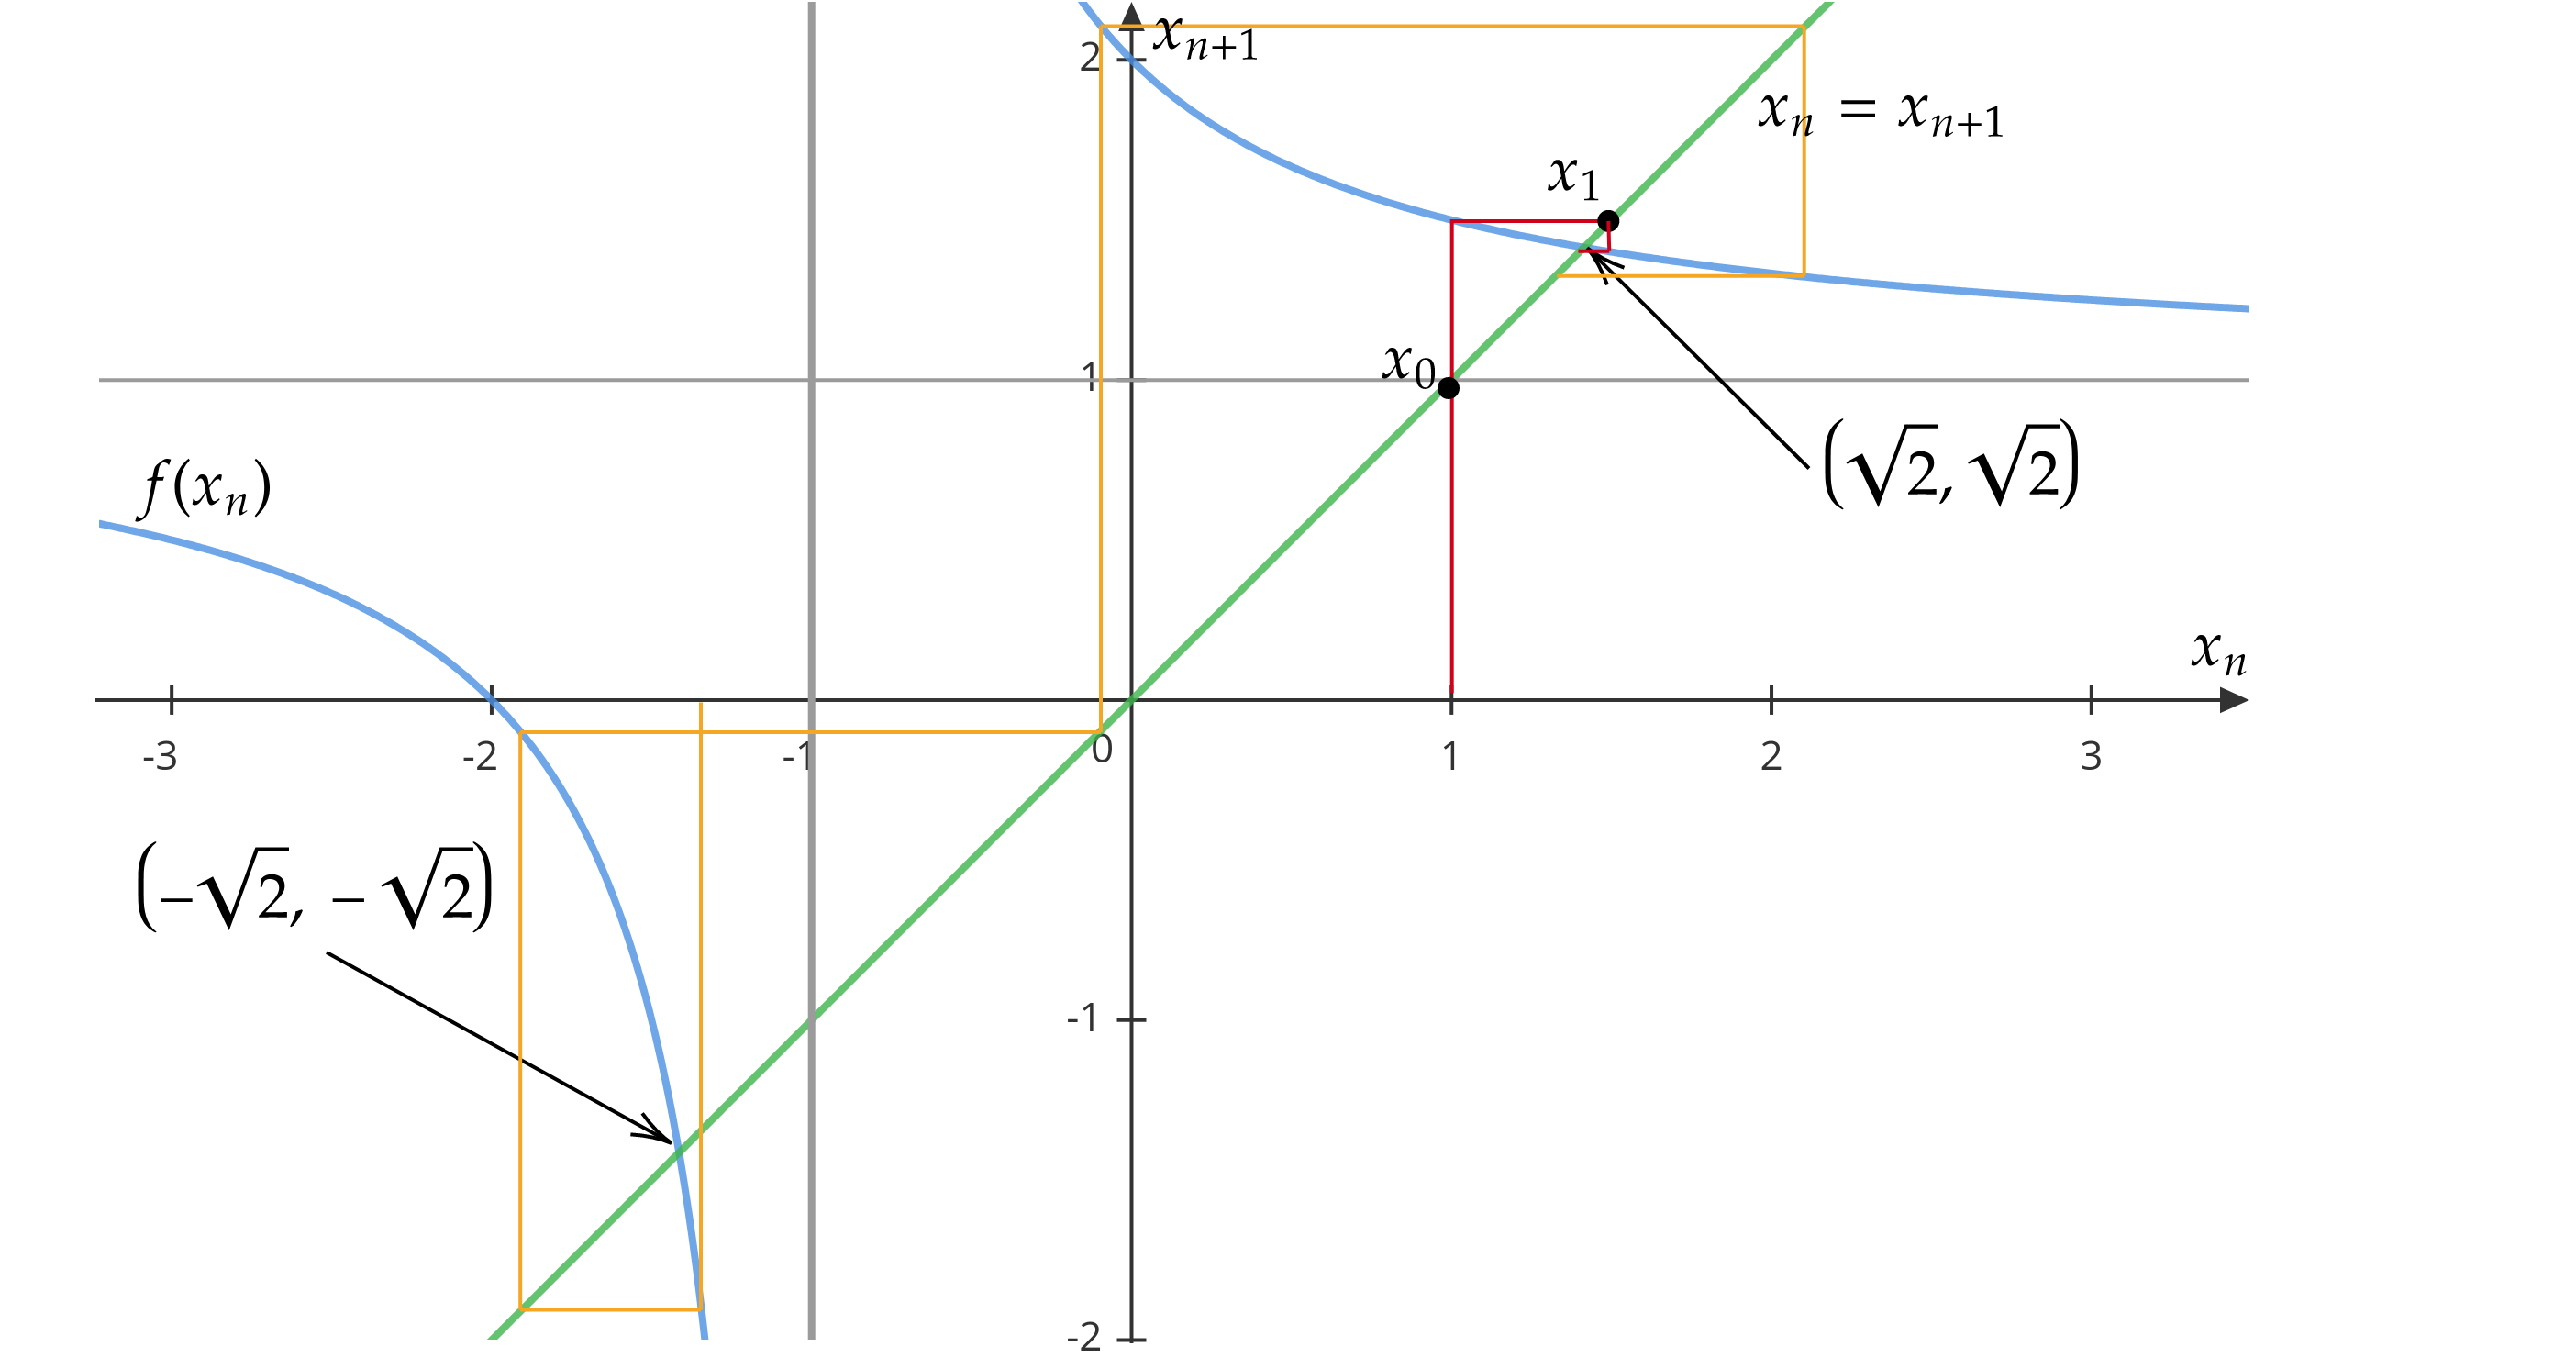
\includegraphics[width = 1\textwidth]{fig9.png}
    \caption{График функции перехода и тождественной функции. Они пересекаются в двух точках, указанных на рисунке. Красной линией обозначен путь последовательности, если стартовать из точки $x_0=1$, желтым отмечен путь последовательности, если начинать с $x_0 < 0$.}
    \label{fig:9}
\end{figure}
Точки $x_n = \pm \sqrt{2}$ являются стационарными точками нашей последовательности, то есть если $x_0 = \pm\sqrt{2}$, то и все последующие члены последовательности будут равны $x_0$ (последовательность тривиальным образом сходится). А что будет, если последовательность стартует не со стационарных точек?
\par
Обратимся к случаю, когда последовательность стартует с $1$ ($x_0=1$). Чтобы найти $x_1$ проводим из $x_0$ вертикальную линию до функции перехода, потом из точки пересечения вертикальной линии с графиком функции перехода проводим горизонтальную линию до графика идентичной функции. Абсцисса полученной точки на диагонали соответствует $x_1$. Дальше продолжаем эти действия и получаем скручивающуюся внутрь спираль, стягивающуюся к стационарной точке $\sqrt{2}$. Таким образом, мы получаем, что последовательность сходится к стационарной точке $\sqrt{2}$.
\par
Посмотрим, что будет происходить с последовательностью, если стартовать из точки, близкой к $-\sqrt{2}$. Как видно на рисунке \ref{fig:9}, последовательность опять уходит в область, близкую к стационарной точке $\sqrt{2}$ и мы снова получаем стягивающуюся к данной стационарной точке спираль. Для большей наглядности можно выписать значения последовательности, которая начинается с точки, близкой к точке $-\sqrt{2}$:
\begin{equation}
    x_0 = -\dfrac{10}{7}, x_1 = - \dfrac{4}{3}, x_2 = -2, x_3 = 0, x_4 = 2, x_5 = \dfrac{4}{3}, x_6 = \dfrac{10}{7}, \ldots
\end{equation}
Видно, что последовательность приходит к значениям, близким к $\sqrt{2}$.
\par
В чём же причина различия стационарных точек $\sqrt{2}$ и $-\sqrt{2}$? Интуиция подсказывает, что дело заключается в наклоне графика функции перехода в данной стационарной точке. Так в точке $\sqrt{2}$ наклон малый, а в точке $-\sqrt{2}$ наклон большой. Это наталкивает на следующий критерий.
\begin{theorem}
Если в данной стационарной точке производная \cite{dif} функции перехода меньше единицы по модулю, то последовательность будет сходится к данной стационарной точке, если же производная больше единицы по абсолютному значению, то последовательность будет расходиться от данной стационарной точки.
\end{theorem}
Стационарные точки, к которым последовательность сходится, называют \emph{устойчивыми}. Стационарные точки, от которых последовательность расходится, называют \emph{неустойчивыми}. Более строго все эти понятия рассмотрены в теории динамических систем \cite{bal}.

\section{"Хаотическое"{} поведение рекуррентной последовательности}
Рассмтрим более сложный пример рекуррентной последовательности. Пускай функция перехода задана следующим образом:
\begin{equation}
    f\qty(x_{n}) = 2x_n^2 - 1.
\end{equation}
Тогда стационарные точки будут находится в $1$ и $-1/2$ (для их нахождения нужно решить $f\qty(x) = x$). Обе стационарные точки являются неустойчивыми, так как производная функции перехода в них больше $1$ по абсолютному значению:
\begin{equation}
    f'\qty(x) = 4x, \quad f'\qty(1) = 4 > 1, \quad  f'\qty(-\dfrac{1}{2}) = -2 < -1.
\end{equation}
Если стартовать из точки вне интервала ($-1,1$), то последовательность будет расходится. Если же стартовать из точки внутри интервала, то две неустойчивых стационарных точки будут отталкивать последовательность от границ интервала, а внутри будет наблюдаться движение, похожее на "{}хаотическое"{} (см. рис. \ref{fig:10}).
\begin{figure}[ht]
    \centering
    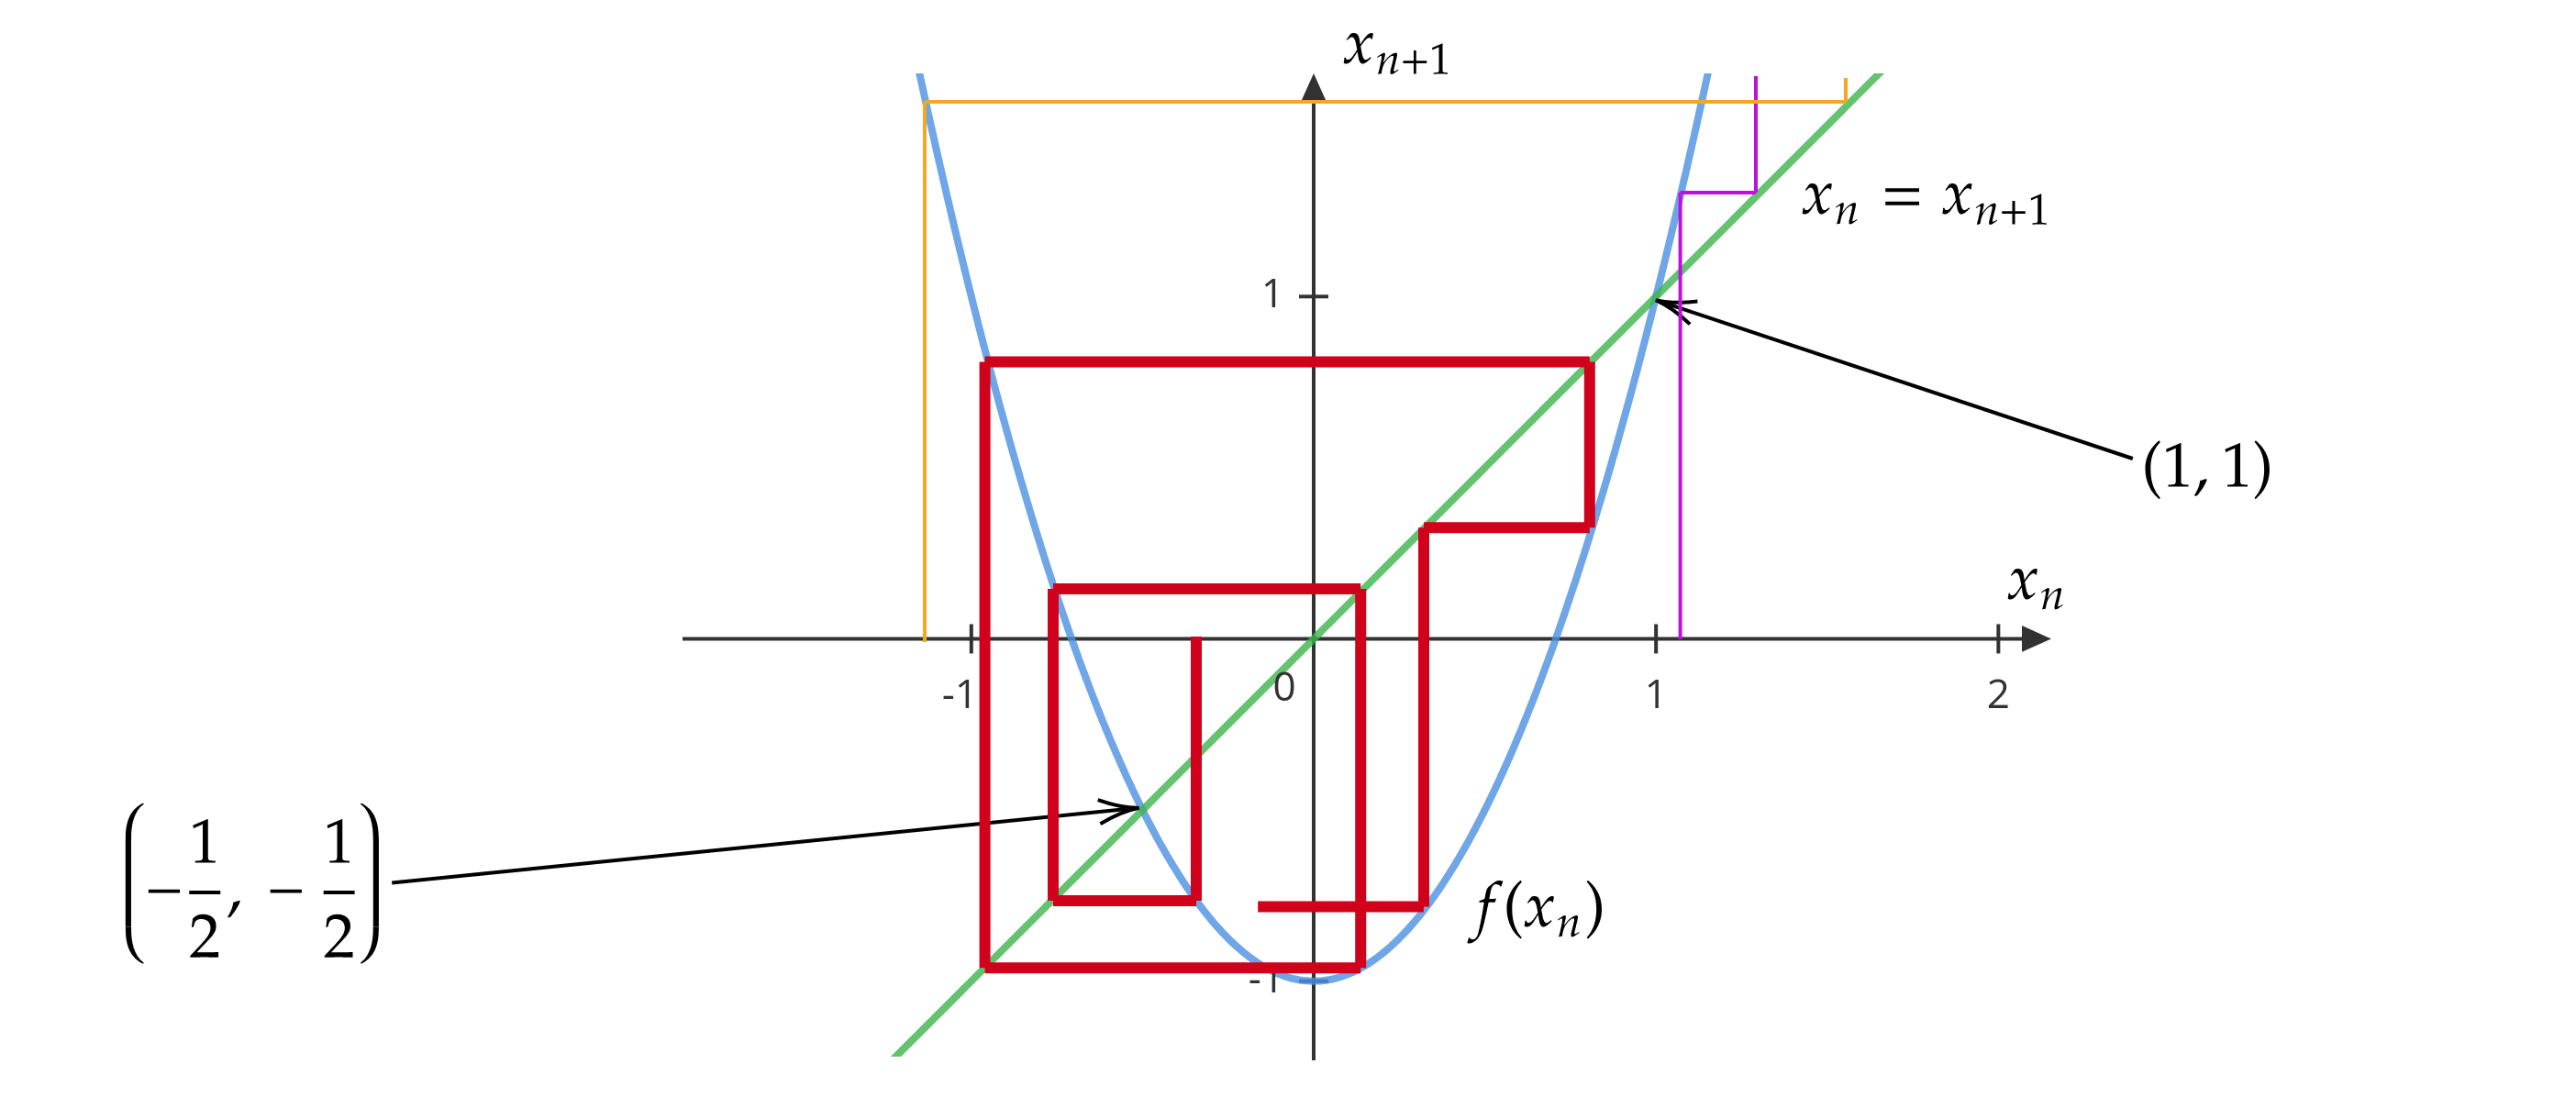
\includegraphics[width = 1\textwidth]{fig10.png}
    \caption{График функции перехода и тождественной функции. Они пересекаются в двух точках, указанных на рисунке. Красной линией обозначен путь последовательности, если стартовать из точки внутри интервала $(-1,1)$, желтым отмечен путь последовательности, если начинать с $x_0 < -1$, фиолетовым обозначено движение последовательности при старте с $x_0 > 1$.}
    \label{fig:10}
\end{figure}
Попробуем дать математическое объяснение данного явления. Для этого введём замену переменых
\begin{equation}
    x_n = \cos{y_n}.
\end{equation}
Нас будет интересовать только интервал $x\in (-1,1)$, поэтому выбор такой замены может иметь право на жизнь. Посмотрим куда отобразится функцией перехода $y_n$:
\begin{equation}
    x_{n+1} = \cos{y_{n+1}} = 2 \cos^2{y_n} - 1 = \cos{2y_n}.
\end{equation}
Значит, $y_{n+1} = 2y_n$. Это функция перехода для последовательности игриков. Через начальный элемент последовательности это можно записать:
\begin{equation}
    y_n = y_0 2^n.
\end{equation}
Лучше всего визуализировать данную последовательность на единичной окружности (см. рис. \ref{fig:11}). Точки последовательности всюду плотно заполняют окружность. Имеется несколько стационарных точек. Прежде всего это точка $y_0 = 0$, попав в неё однажды, последовательность останется в ней на всегда. Кроме того, есть две точки $2\pi/3$ и $-2\pi/3$, точка на окружности переходит из одной из этих точек в другую, при этом косинус остаётся постоянным, поэтому для последовательности $x_n$ данные значения $y_n$ являются стационарными.
\begin{figure}[ht]
    \centering
    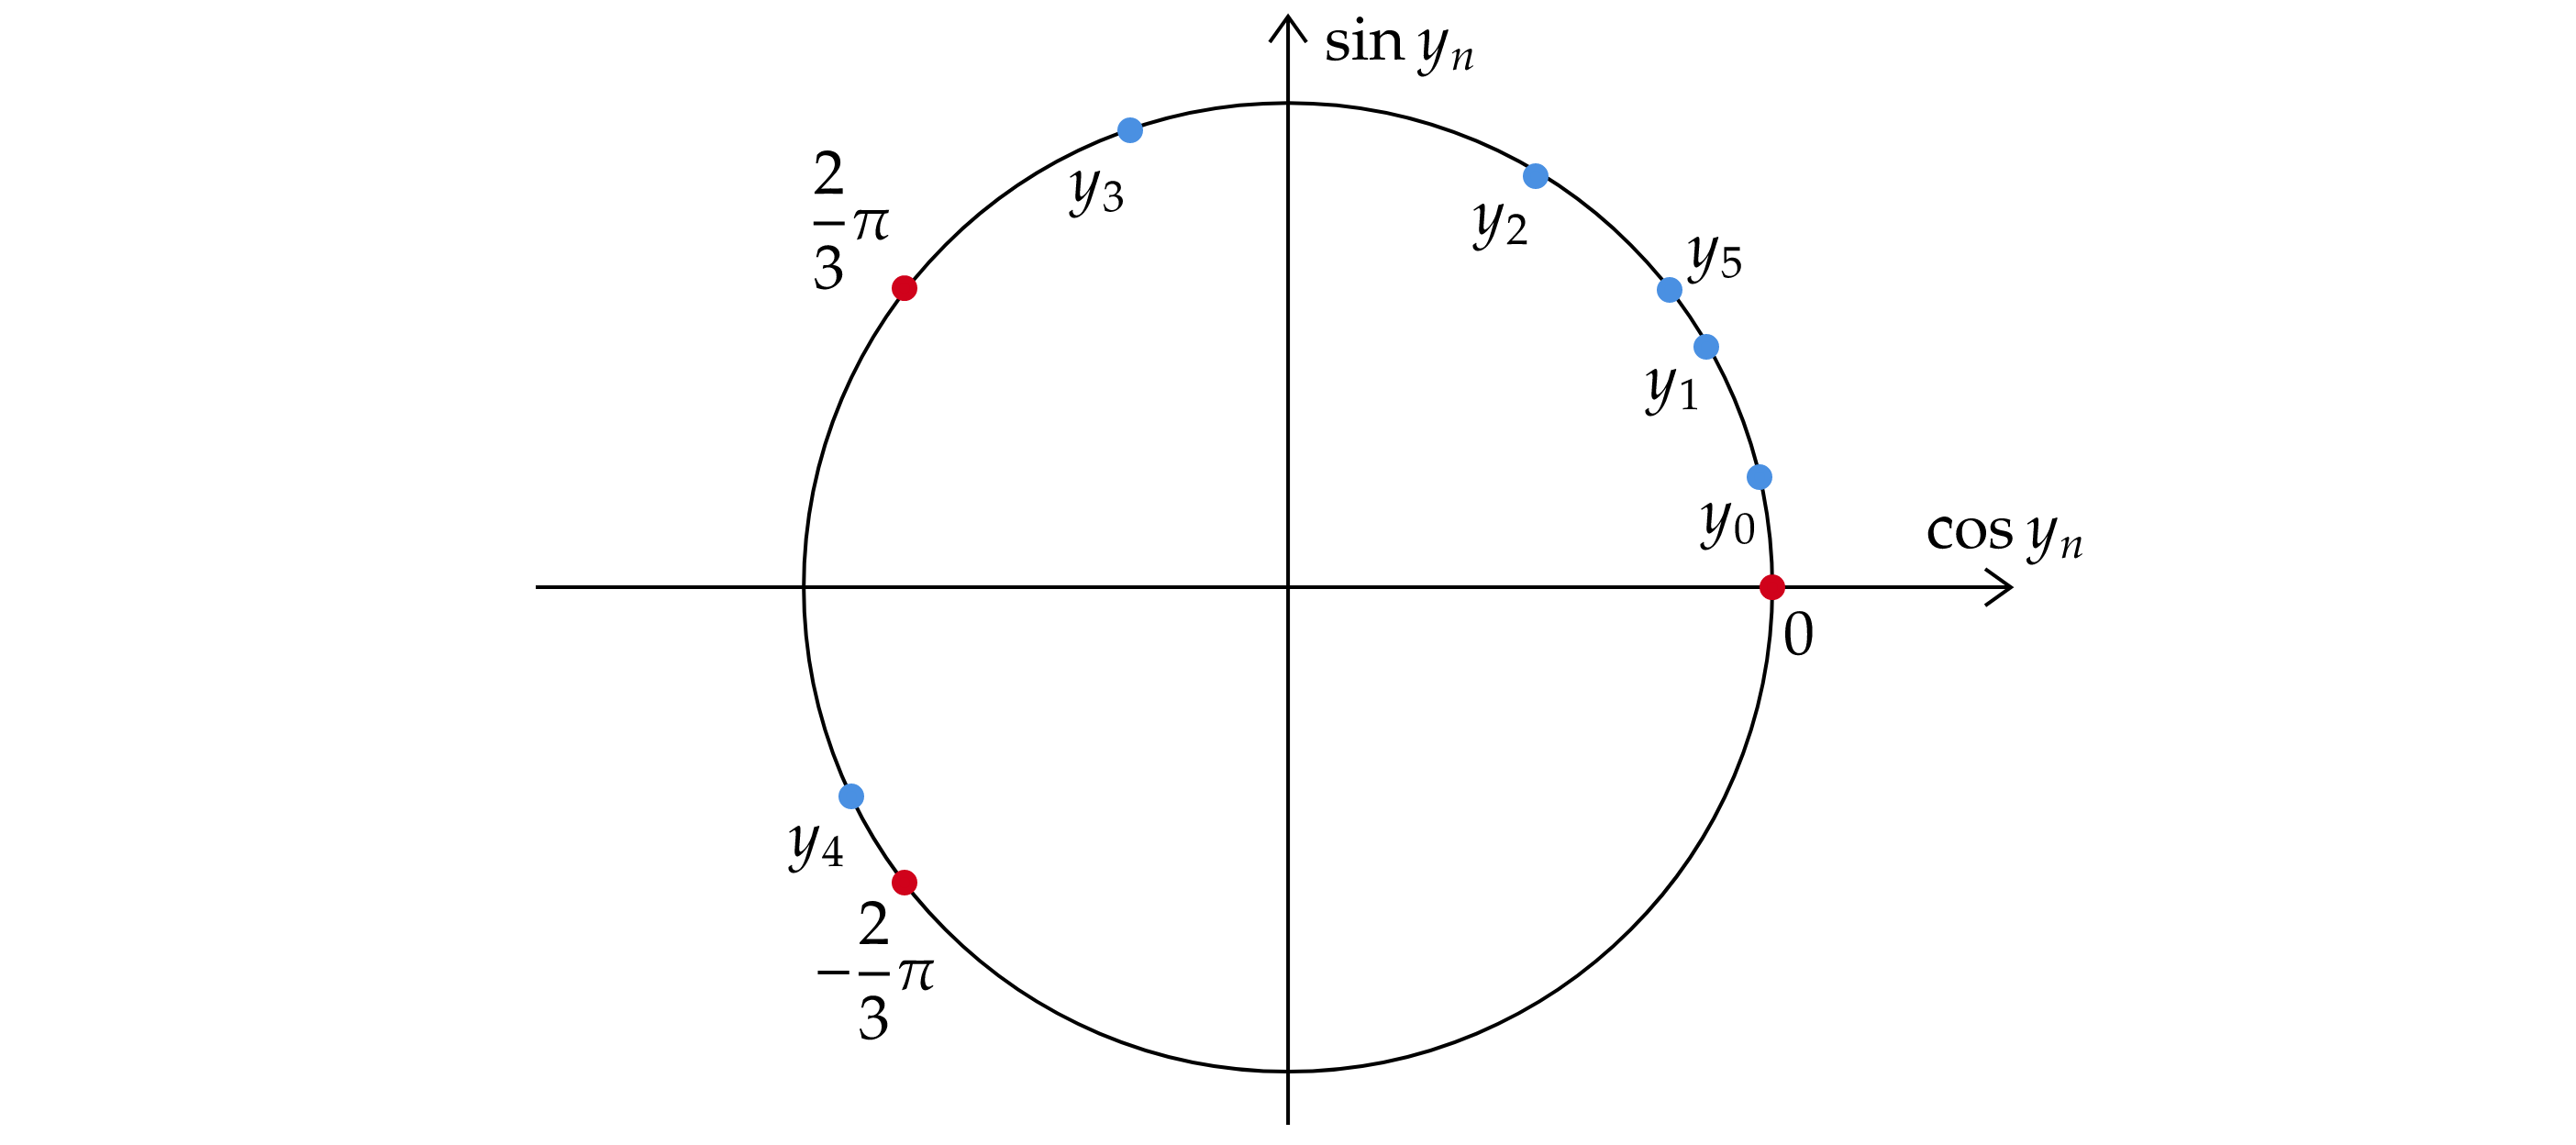
\includegraphics[width = 1\textwidth]{fig11.png}
    \caption{График единичной окружности для иллюстрации последовательности $y_n$. Красным обозначены стационарные точки. Если за $y_0$ выбрано число, которое не является числом $\pi$, умноженным на рациональное число, то элементы полученной последовательности будут всюду плотно заполнять окружность. Можно это проиллюстрировать, откладывая сперва элементы последовательности на прямой, а потом начать наматывать прямую на окружность, тогда из\--за того, что длина окружности кратна $\pi$, а элементы последовательности нет, ни один элемент последовательность не наложиться на другой элемент при накручивании, а так как членов последовательности бесконечно много, в то время как длина круга конечна, то элементы последовательности разместяться на окружности единственным возможным способом~\----~будут всюду плотно её заполнять.}
    \label{fig:11}
\end{figure}
\par
Можно заметить, что точки $y_0$, кратные $2\pi$, делённым на какую\--то степень двойки, пораждают последовательности сходящиеся в нуль за конечное число отображений. Если же стартовать из точек $y_0$, кратных $2\pi/3$, делённым на какую\--то степень двойки, то мы так же придём за конечное число отображений к стационарной точке $x = -1/2$. Таким образом на интервале $\qty(-1,1)$ бесконечно много всюду плотных точек, пораждающих сходящиеся в стационарные точки за конечное число итераций последовательности.
\par
Однако кроме данных точек существуют все остальные точки, стартовав с которых, последовательность не прийдёт ни в какое стационарное состояние и будет бесконечно долго совершать хаотически движения по интервалу $\qty(-1,1)$.


\medskip 
\begin{thebibliography}{9}
\bibitem{pif}
Савватеев А., Тонис А., \textit{Введение в математический анализ},
\\\texttt{\url{https://enabla.com/ru/pub/611}} (Версия от 25.07.2021)

\bibitem{bal}
Балакин А. А., \textit{Элементы КАМ\--теории. Глобальный хаос},
\\\texttt{\url{https://enabla.com/ru/set/12/pub/223}} (Версия от 06.08.2021)

\bibitem{sum}
Савватеев А., Тонис А., \textit{Ряды с неотрицательными слагаемыми},
\\\texttt{\url{https://enabla.com/ru/pub/613}} (Версия от 01.08.2021)

\bibitem{dif}
Wikipedia, \textit{Производная функции},
\href{https://ru.wikipedia.org/wiki/\%D0\%9F\%D1\%80\%D0\%BE\%D0\%B8\%D0\%B7\%D0\%B2\%D0\%BE\%D0\%B4\%D0\%BD\%D0\%B0\%D1\%8F_\%D1\%84\%D1\%83\%D0\%BD\%D0\%BA\%D1\%86\%D0\%B8\%D0\%B8}{https://ru.wikipedia.org/wiki/Производная\_функции} (Версия от 06.08.2021)

\end{thebibliography}
\end{document}